%!TEX root = main.tex

\section{$L$-level Recommendation Policy}
\label{sec:llevel}
In this section, we give an overview of how we extend our 3-level policy to an $L$-level policy for $L > 3$ in order to achieve better regret. In Theorem \ref{thm:llevel-1}, we show our $L$-level policy. We can achieve nearly optimal regret $O(T^{1/2} polylog(T))$ with $O(\log\log(T))$ levels.
\begin{theorem}
\label{thm:llevel-1}
For any $L > 3$, we have an $L$-level recommendation policy with expected regret \\$O\left(T^{2^{L-1}/(2^L-1)} polylog(T) \right)$. In particular, we have an $O(\log\log(T))$-level recommendation policy with expected regret $O(T^{1/2} polylog(T))$. 
\end{theorem}

In Theorem \ref{thm:llevel-2}, we show a recommendation policy with instance-dependent regret guarantee. This policy has the same structure as the one in Theorem \ref{thm:llevel-1} but different parameters. Its expected regret depends on $\Delta$ which is the difference between the largest mean and second largest mean of arms and its construction does not depend on $\Delta$. Its regret bound outperforms the one in Theorem \ref{thm:llevel-1} when $\Delta$ is much bigger than $T^{-1/2}$. The only downside is that this policy requires more levels, i.e. $O(\log(T)/\log\log(T))$ levels. It also has the property that each agent observes a good fraction of history till its round. 

\begin{theorem}
\label{thm:llevel-2}
 We have an $O(\log(T)/\log\log(T))$-level recommendation policy with expected regret $O(\min(1/\Delta, T^{1/2})polylog(T))$. Here $\Delta$ is the difference between the largest mean and second largest mean of arms. The recommendation policy does not depend on $\Delta$. Moreover, agent in round $t$ observes a subhistory of size at least $\Omega( \lfloor t/polylog(T)\rfloor)$. 
\end{theorem}

Detailed proofs and discussions of Theorem \ref{thm:llevel-1} and Theorem \ref{thm:llevel-2} can be found in Appendix \ref{sec:llevel-details}. Similarly as Section \ref{sec:3level}, we first prove them in the case of 2 arms (Theorem \ref{thm:llevel} and Corollary \ref{cor:llevel}). We then extend them to the case of constant number of arms (Theorem \ref{thm:constarm}).

The main idea of extending from 3-level to $L$-level is that instead of using the second level as one ``check-point'', we use more levels to have multiple ``check points''.  Some new challenges appear in this process. Here give an overview of the additional techniques we use to get our $L$-level results. 

\xhdr{Connecting structures between levels.} In our 3-level policy, the second level has $S = \Theta(\log(T))$ groups. We do so to ensure that in the small gap case, with high probability, both arms are pulled enough times in the second level. The argument relies on the fact that agents in different second-level groups observe disjoint histories of the first level and the independent randomness in first level groups guarantee each arm $a$ to have a ``lucky'' second-level group such that agents in that group all pull arm $a$ with high probability. 

Simply generalizing this idea to an $L$-level policy would give us a $S$-ary tree like structure in the info graph. It incurs an extra $S^L$ factor in the expected regret. If we use $\log\log(T)$ levels as in Theorem \ref{thm:llevel-1}, this factor would be $\Omega\left(\log(T)^{\log\log(T)}\right)$ which is super poly-logarithmic. If we use $\log(T)/\log\log(T)$ levels as in Theorem \ref{thm:llevel-2}, this factor goes up to polynomial in $T$. 

In order to avoid this undesirable factor, we design a slightly different connecting structure in our $L$-level policy. The key observation is that, for any level $l \in \{3,...,L-1\}$, we do want agents in different $l$-th level groups to see disjoint histories of the $(l-1)$-th level to ensure that there is some ``lucky'' group for each arm $a$ when arm $a$'s mean is close enough to the best arm. However, it does not matter much if these agents see the same history of levels below $l-1$ because group sizes in lower levels are much smaller than group sizes in higher levels and the independent randomness in level $l-1$ is sufficient.

To explain the figure..
\begin{figure}[H]
\centering
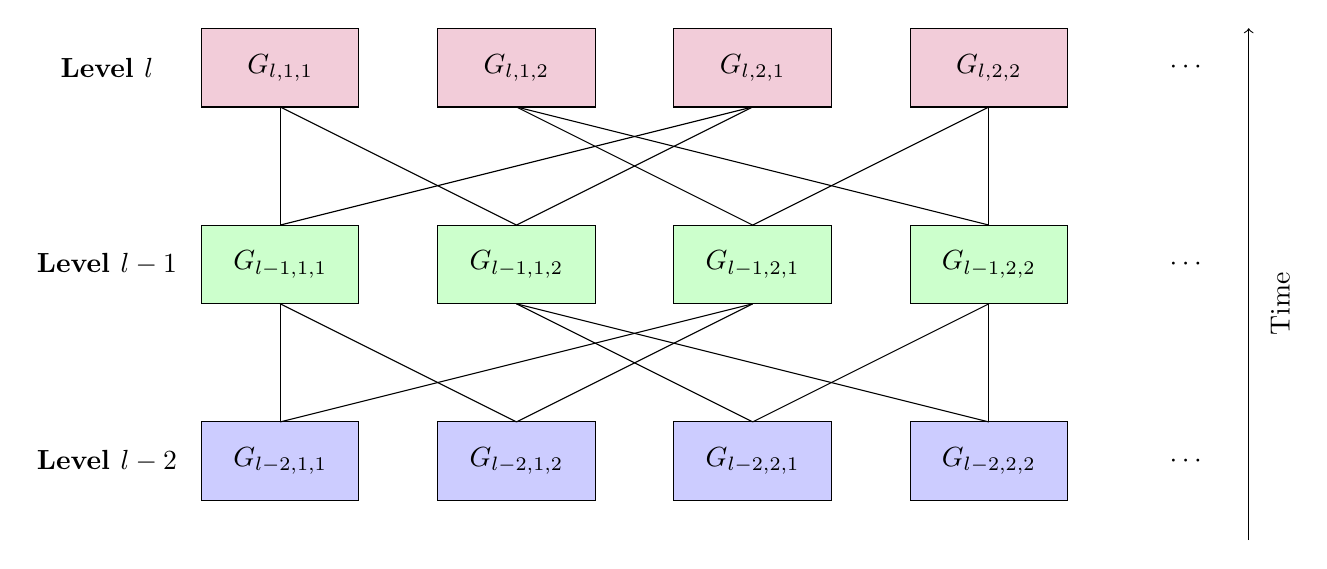
\begin{tikzpicture}  
 \foreach \x in {0,3,6,9}
 {
 \filldraw[fill=purple!20!white]
 (\x+0,7.5)--(\x+2,7.5)--(\x+2,8.5)--(\x+0,8.5)--cycle;
 \filldraw[fill=green!20!white]
 (\x+0,5)--(\x+2,5)--(\x+2,6)--(\x+0,6)--cycle;
 \filldraw[fill=blue!20!white]
 (\x+0,2.5)--(\x+2,2.5)--(\x+2,3.5)--(\x+0,3.5)--cycle;
 }
\foreach \y in {2.5,5,7.5}
{
  \node at (12.5,\y+0.5){$\cdots$};
} 


\foreach \y in {3.5,6}
{
  \draw (1,\y) -- (1,\y+1.5);
  \draw (1,\y) -- (7,\y+1.5);
  
  \draw (4,\y) -- (1,\y+1.5);
  \draw (4,\y) -- (7,\y+1.5);
  
  
  \draw (7,\y) -- (4,\y+1.5);
  \draw (7,\y) -- (10,\y+1.5);
  
  
  \draw (10,\y) -- (4,\y+1.5);
  \draw (10,\y) -- (10,\y+1.5);
} 

\foreach \u in {1,2}
{
	\foreach \v in {1,2}
	{
	\pgfmathsetmacro{\x}{((\u-1)*2+(\v-1))*3};
	\pgfmathsetmacro{\xa}{((\u-1))*3};
	\pgfmathsetmacro{\xb}{(2+(\u-1))*3};
   \node at(\x+1,8){$G_{l,\u,\v}$};
   \node at(\x+1,5.5){$G_{l-1,\u,\v}$};
   \node at(\x+1,3){$G_{l-2,\u,\v}$};
	}
}


  \node at(-1.2,3){\textbf{Level $l-2$}};
  \node at(-1.2,5.5){\textbf{Level $l-1$}};
  \node at(-1.2,8){\textbf{Level $l$}};
  \draw[->] (13.3,2)--(13.3,8.5);
  \node at(13.7,5)[ rotate=90]{Time};

\end{tikzpicture}
\caption{Connectiing structures between levels for the $L$-level policy.}
\label{fig:llevel-connecting}
\end{figure}
\xhdr{Additional groups for boundary cases.}